\chapter{Conjunto de datos} 

Se ha hecho uso de un conjunto de datos generados por la International Skin Imaging Collaboration (ISIC) en donde las imágenes provienen de las siguientes fuentes: Hospital Clínic de Barcelona, Medical University of Vienna, Memorial Sloan Kettering Cancer Center, Melanoma Institute Australia, University of Queensland y University of Athens Escuela de Medicina \citep{isic-archive}.

Este conjunto de datos contiene 33.126 imágenes de entrenamiento dermatoscópicas de lesiones cutáneas benignas y malignas únicas de más de 2.000 pacientes. Cada imagen se asocia con una de estas personas mediante un identificador de paciente único. Todos los diagnósticos malignos se han confirmado mediante histopatología, y los diagnósticos benignos se han confirmado mediante el acuerdo de expertos, el seguimiento longitudinal o la histopatología. 

El conjunto de datos fue seleccionado para el SIIM-ISIC Melanoma Classification Challenge organizado en Kaggle durante el verano de 2020 \cite{kaggle}.


\section{Análisis de datos}

Las imágenes se proporcionan en formato DICOM, JPEG y TFRecord. Los metadatos también se proporcionan en archivos CSV.

\begin{figure}[htbp]
    \centering
    \textbf{}\par\medskip
    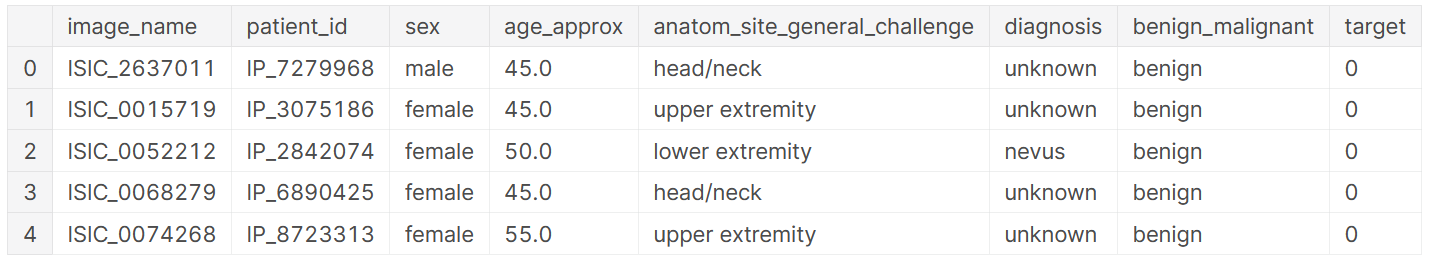
\includegraphics[scale=0.5]{3/figures/metadata/datos_tabulares.PNG}
    \caption{Primeras cinco filas de los datos tabulares de entrenamiento}
    \label{tabular_data}
\end{figure}

El propósito de la competición consiste en predecir un objetivo binario para cada imagen. El modelo debe predecir la probabilidad entre 0.0 y 1.0 de que la lesión en la imagen sea maligna. En los datos de entrenamiento, "train.csv", el valor 0 denota benigno y 1 indica maligno.

\begin{figure}[htbp]
    \centering
    \textbf{}\par\medskip
    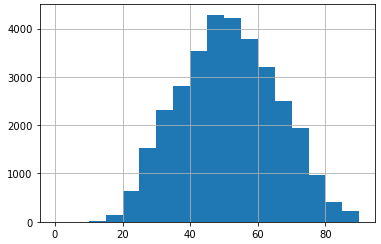
\includegraphics[scale=0.65]{3/figures/metadata/age_count.PNG}
    \caption{Edades}
    \label{age_count}
\end{figure}

\begin{figure}[htbp]
    \centering
    \textbf{}\par\medskip
    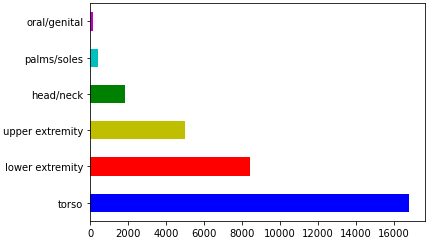
\includegraphics[scale=0.65]{3/figures/metadata/anatom_site_general_count.PNG}
    \caption{Parte del cuerpo}
    \label{anatom_site_general_count}
\end{figure}

\begin{figure}[htbp]
    \centering
    \textbf{}\par\medskip
    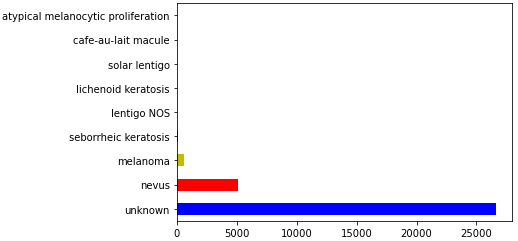
\includegraphics[scale=0.65]{3/figures/metadata/diagnosis_count.PNG}
    \caption{Diagnosis}
    \label{diagnosis_count}
\end{figure}

\begin{figure}[htbp]
    \centering
    \textbf{}\par\medskip
    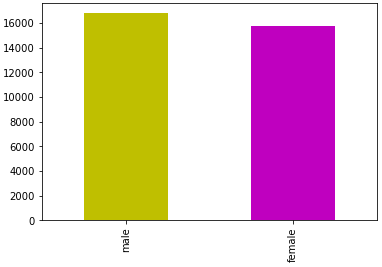
\includegraphics[scale=0.65]{3/figures/metadata/gender_count.PNG}
    \caption{Género}
    \label{gender_count}
\end{figure}

\begin{figure}[htbp]
    \centering
    \textbf{}\par\medskip
    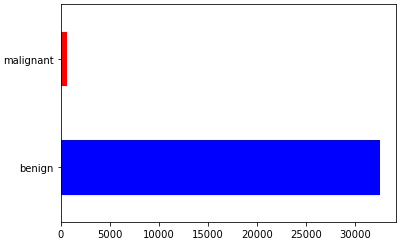
\includegraphics[scale=0.65]{3/figures/metadata/imbalance_class.PNG}
    \caption{Desbalanceo de clases}
    \label{imbalance_class}
\end{figure}

%\newpage

\subsection{Desbalanceo de datos}

La mayoría de los modelos utilizados para aprender de un conjunto de datos de las métricas utilizadas para evaluar esos modelos se diseñaron en torno al supuesto que la distribución de las clases sea igual. En cambio, cuando estas están desequilibrados, muchos algoritmos de aprendizaje automático fallan y las métricas utilizadas para evaluar esos modelos, como la precisión de la clasificación (o \emph{accuracy}), se vuelven engañosos \cite{imbalanced-classification}.

Como se observa en la figura \ref{imbalance_class}, existe un problema donde la distribución de ejemplos en las clases conocidas no está balanceada. Esto hace que la clase minoritaria sea más difícil de predecir porque hay pocos ejemplos de esta clase, por definición. Esto significa que es más difícil para un modelo aprender las características de los ejemplos de esta clase, y para diferenciar ejemplos de esta clase de la clase mayoritaria.

Como consecuencia, la mayoría de los modelos tienen un rendimiento predictivo deficiente, específicamente para la clase minoritaria. Esto presenta un inconveniente ya que la clase minoritaria (cáncer maligno) es más importante de clasificar correctamente y, por lo tanto, el problema es más sensible a los errores de clasificación para la clase minoritaria que la clase mayoritaria.


Para intentar solucionar este problema, se han propuesto modificaciones a los algoritmos existentes para hacer que sean útiles para la clasificación desequilibrada, la selección de métricas de rendimiento y nuevas técnicas de preparación de datos y algoritmos de modelado.

\subsubsection{Data augmentation}
Un enfoque para abordar los conjuntos de datos desequilibrados es sobremuestrear la clase minoritaria en el conjunto de datos de entrenamiento antes de entrenar el modelo. Esto implica la duplicación de ejemplos en la clase minoritaria, aunque estos ejemplos no agregue ninguna información nueva. En cambio, se pueden sintetizar nuevos ejemplos a partir de los ejemplos existentes \cite{imbalanced-classification}. 

Este es un tipo de aumento de datos para la clase minoritaria y se refiere como \emph{Synthetic Minority Oversampling Technique} (o SMOTE). Esta técnica fue descrita por Nitesh Chawla y col. en su artículo \cite{SMOTE}.

EJEMPLOS DEL CONJUNTO DE DATOS (sobremuestreo)...

La mayor parte de la atención de los métodos de muestreo para la clasificación se basa en el sobremuestreo de la clase minoritaria. Sin embargo, un conjunto de técnicas ha sido desarrollado para submuestrear la clase mayoritaria que se puede utilizar junto con métodos efectivos de sobremuestreo.

Las técnicas de submuestreo eliminan ejemplos del conjunto de datos de entrenamiento que pertenecen a la clase mayoritaria con el fin de equilibrar mejor la distribución de clases, como por ejemplo, reducir el sesgo de una distribución de clases de 1:100 a 1:10 \cite{imbalanced-classification}. 

La técnica de submuestreo más simple implica la selección aleatoria de ejemplos del clase mayoritaria y eliminándolos del conjunto de datos de entrenamiento. Una extensión de este enfoque es ser más perspicaz con los ejemplos de la clase mayoritaria que se eliminan implicando modelos heurísticos que intentan identificar ejemplos redundantes o ejemplos útiles para no eliminar. Existen muchas técnicas de submuestreo que utilizan este tipo de heurísticas las cuales no se profundizarán en este trabajo.

EJEMPLOS DEL CONJUNTO DE DATOS (submuestreo)...

Normalmente, los métodos de submuestreo se utilizan junto con una técnica de sobremuestreo para la clase minoritaria, y esta combinación a menudo da como resultado mejor rendimiento que el uso de sobremuestreo o submuestreo solo en el conjunto de datos de entrenamiento \cite{imbalanced-classification}.

\subsubsection{Función de pérdida ponderada}

\section{Preprocesamiento de datos}

Se ha redimensionado las imágenes ...

https://stats.stackexchange.com/questions/299292/dropout-makes-performance-worse 